\documentclass{extbook}
\usepackage[papersize={8.5in,11in},top=1in,bottom=1in]{geometry}
\RequirePackage{fix-cm}
\usepackage[T1]{fontenc}
\usepackage{lmodern}
\usepackage{fullpage}
\usepackage{titlesec}
\usepackage{parskip}
\usepackage{float}
\usepackage{url}
\usepackage{hyperref}
\usepackage{graphicx}
\usepackage{tcolorbox}
\usepackage{tabularx}
\usepackage{xcolor}
\usepackage{titlesec}
\usepackage{amsmath}
\usepackage{tcolorbox}
\usepackage{tabularx}

\renewcommand{\contentsname}{Contenido}
\renewcommand{\figurename}{Figura}
%\renewcommand{\listtablename}{Lista de tablas}
\renewcommand{\listfigurename}{Lista de figuras}
\usepackage[fontsize=13.5pt]{fontsize}
\setlength{\parindent}{0pt}

\titleformat{\chapter}[display]
  {\bfseries\huge} % Estilo del título
  {\hfill\Large} % Alineación a la derecha
  {3ex} % Espaciado entre el número del capítulo y el título
  {\vspace{-5cm}\titlerule\vspace{1.5ex}\hfill} % Regla arriba y alineación del título a la derecha
  [\vspace{1ex}\titlerule] % Regla debajo del título


  \makeatletter
  \patchcmd{\chapter}
    {\if@openright\cleardoublepage\else\clearpage\fi}
    {\clearpage}
    {}{}
  \makeatother

  \definecolor{codegreen}{rgb}{0,0.6,0}
  \definecolor{codegray}{rgb}{0.5,0.5,0.5}
  \definecolor{codepurple}{rgb}{0.58,0,0.82}
  \definecolor{backcolour}{rgb}{0.95,0.95,0.92}

\begin{document}
\begin{titlepage}
  \begin{center}
      {\huge \textbf{Universidad Tecnológica de Panamá}}\\
      \vspace{3mm}
      {\Large \textbf{Centro Regional De Veraguas}}

      \begin{figure}[H]
          \centering
          
\includegraphics[scale = 0.07]{Imagenes/UTP/utp.png}
          
\includegraphics[scale = 0.58]{Imagenes/UTP/fisc.png}
      \end{figure}
      {\Large \textbf{Facultad de Ingeniería de Sistemas Computacionales}}\\
      \vspace{5mm}
      
      {\Large \textbf{Curso: Base de Datos II}}\medskip
      
      {\Large \textbf{Profesor: Abdiel Kapell}}

      \rule{\linewidth}{0.75mm}\\
          {\Large \textsc{Parcial 2}} 
      \rule{\linewidth}{0.75mm}\medskip

      {\Large \textbf{Estudiantes}}\\
      \vspace{5mm}
      {\Large \textbf{Elbin Puga, Arland Barrera}}
      \vfill
      {\Huge \textbf{2024}}

  \end{center}
\end{titlepage}
\tableofcontents
\listoffigures
%\listoftables para lista de tablas 
\chapter{Desarrollo}
\section{Diagramas}
\begin{figure}[H]
  \centering
  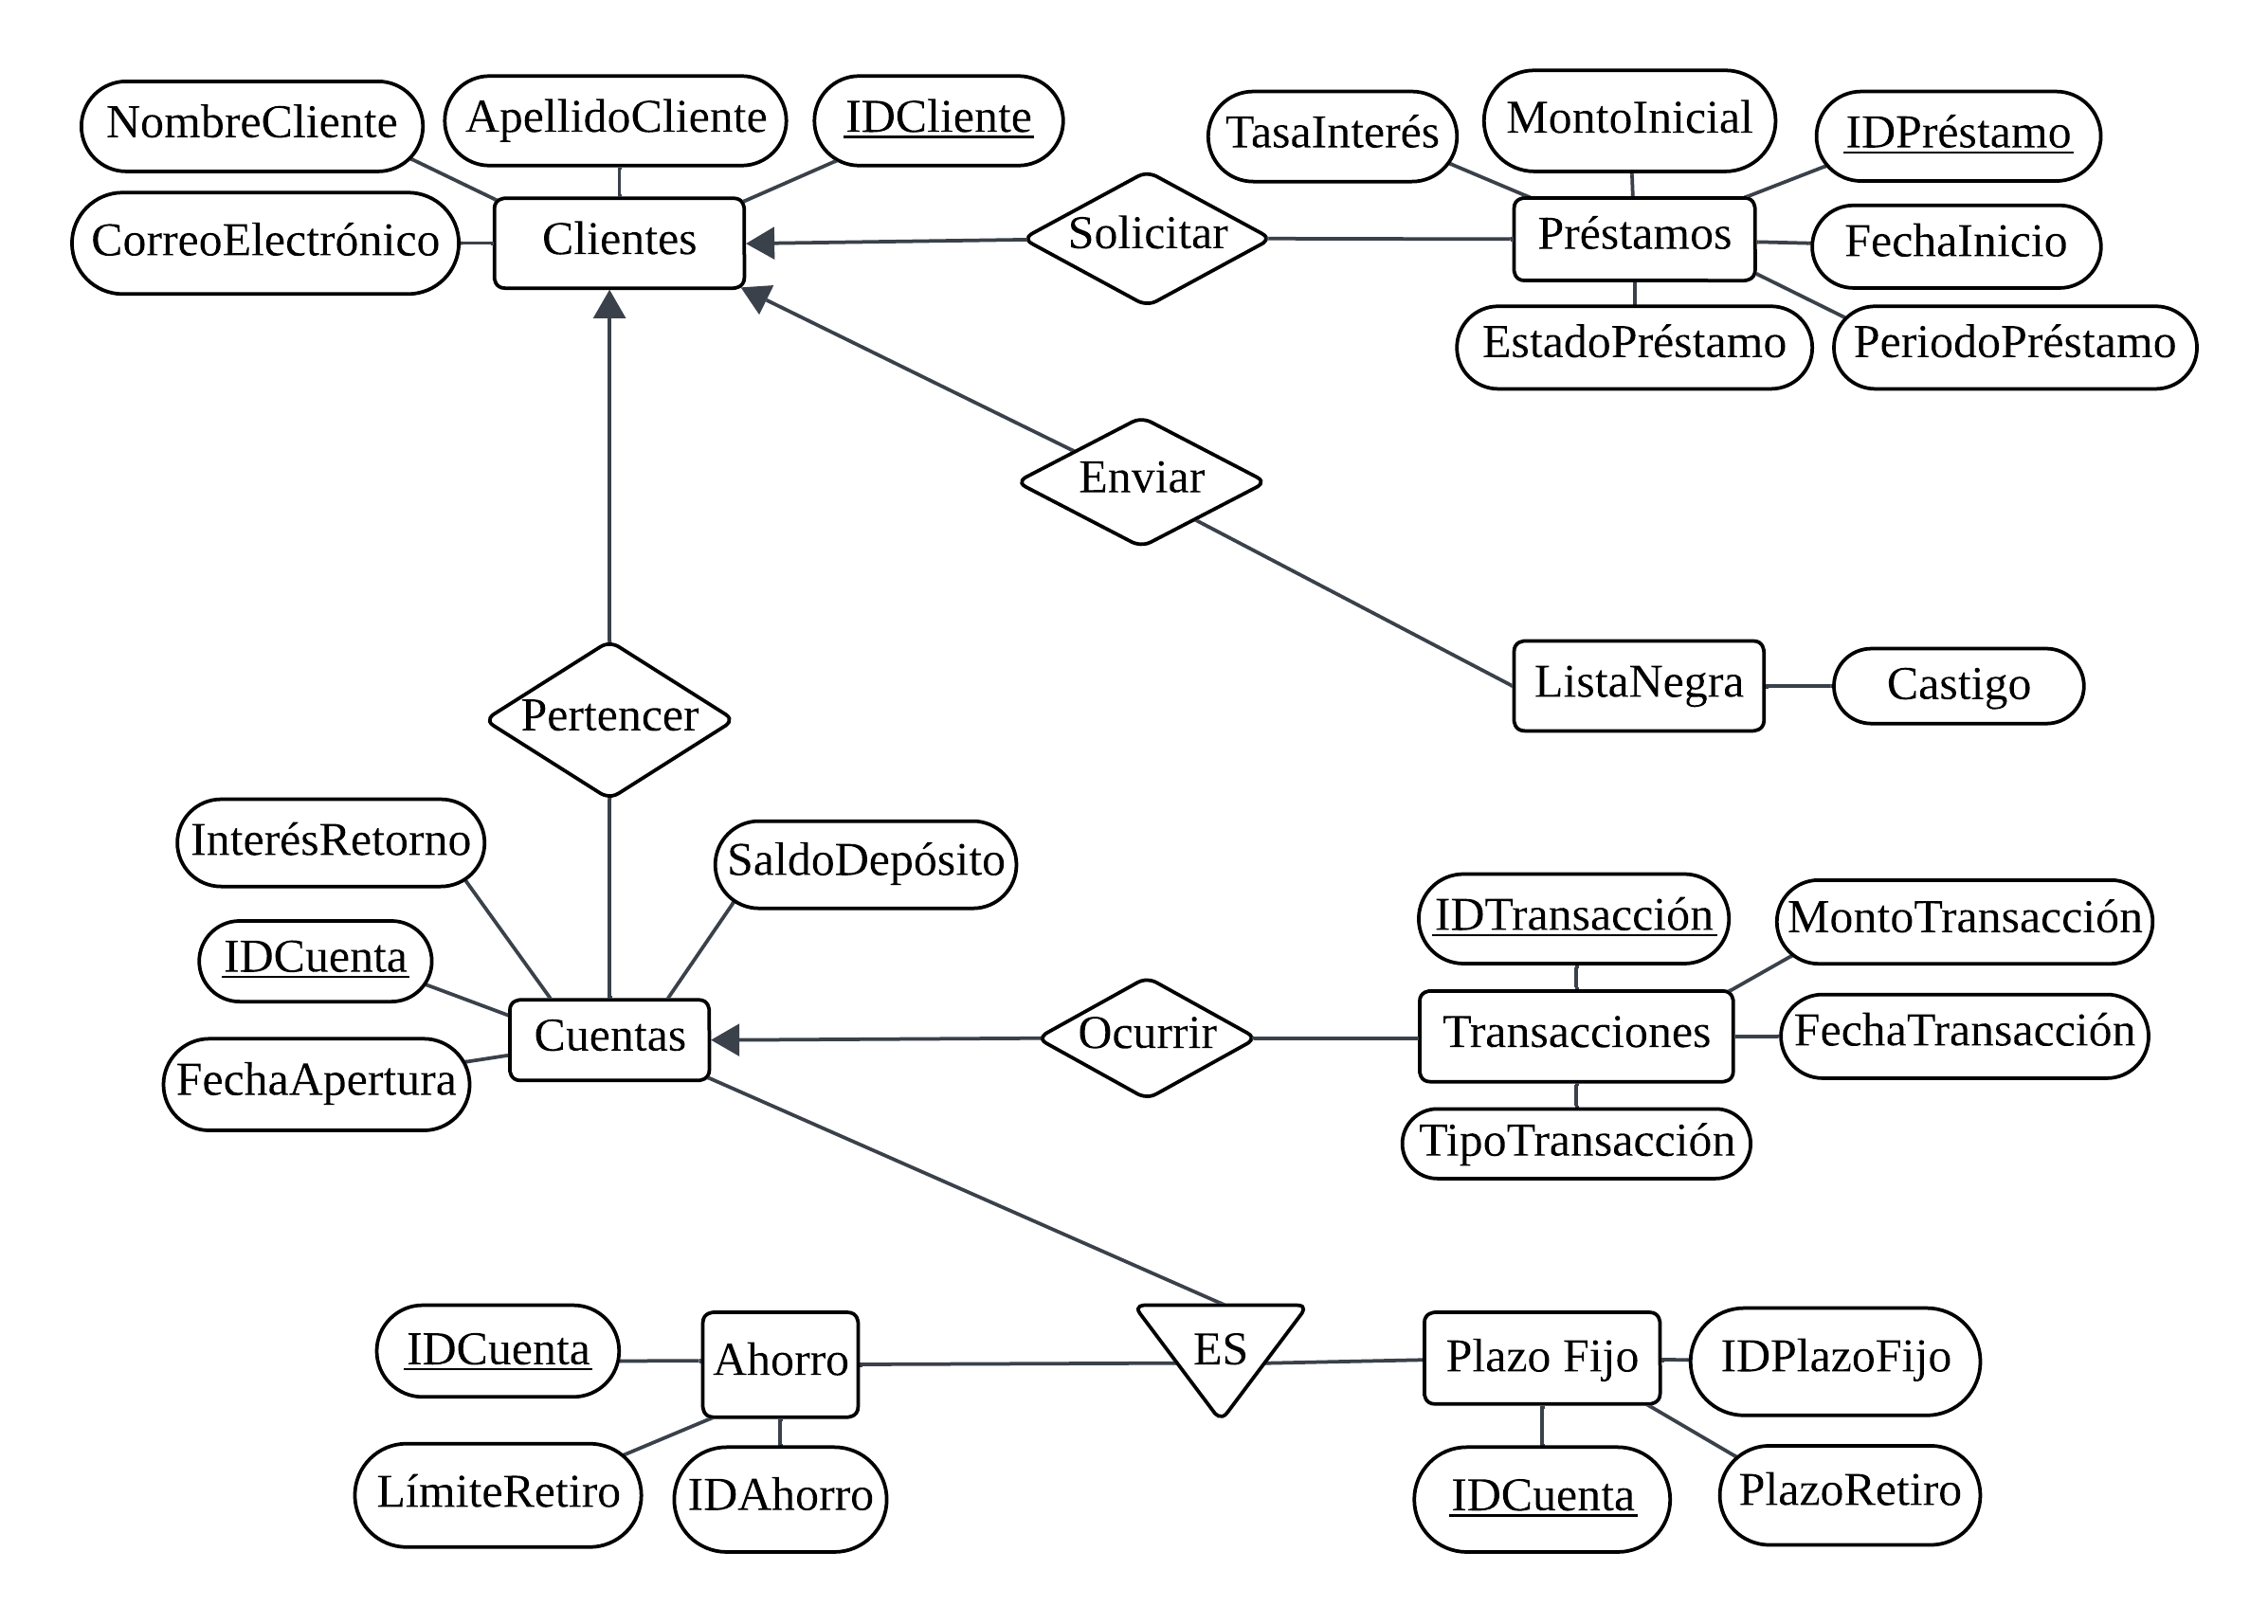
\includegraphics[scale = 0.2]{Imagenes/Diagramas/DERE.png}
  \caption{Diagrama Entidad-Relación}
\end{figure}

\begin{figure}[H]
  \centering
  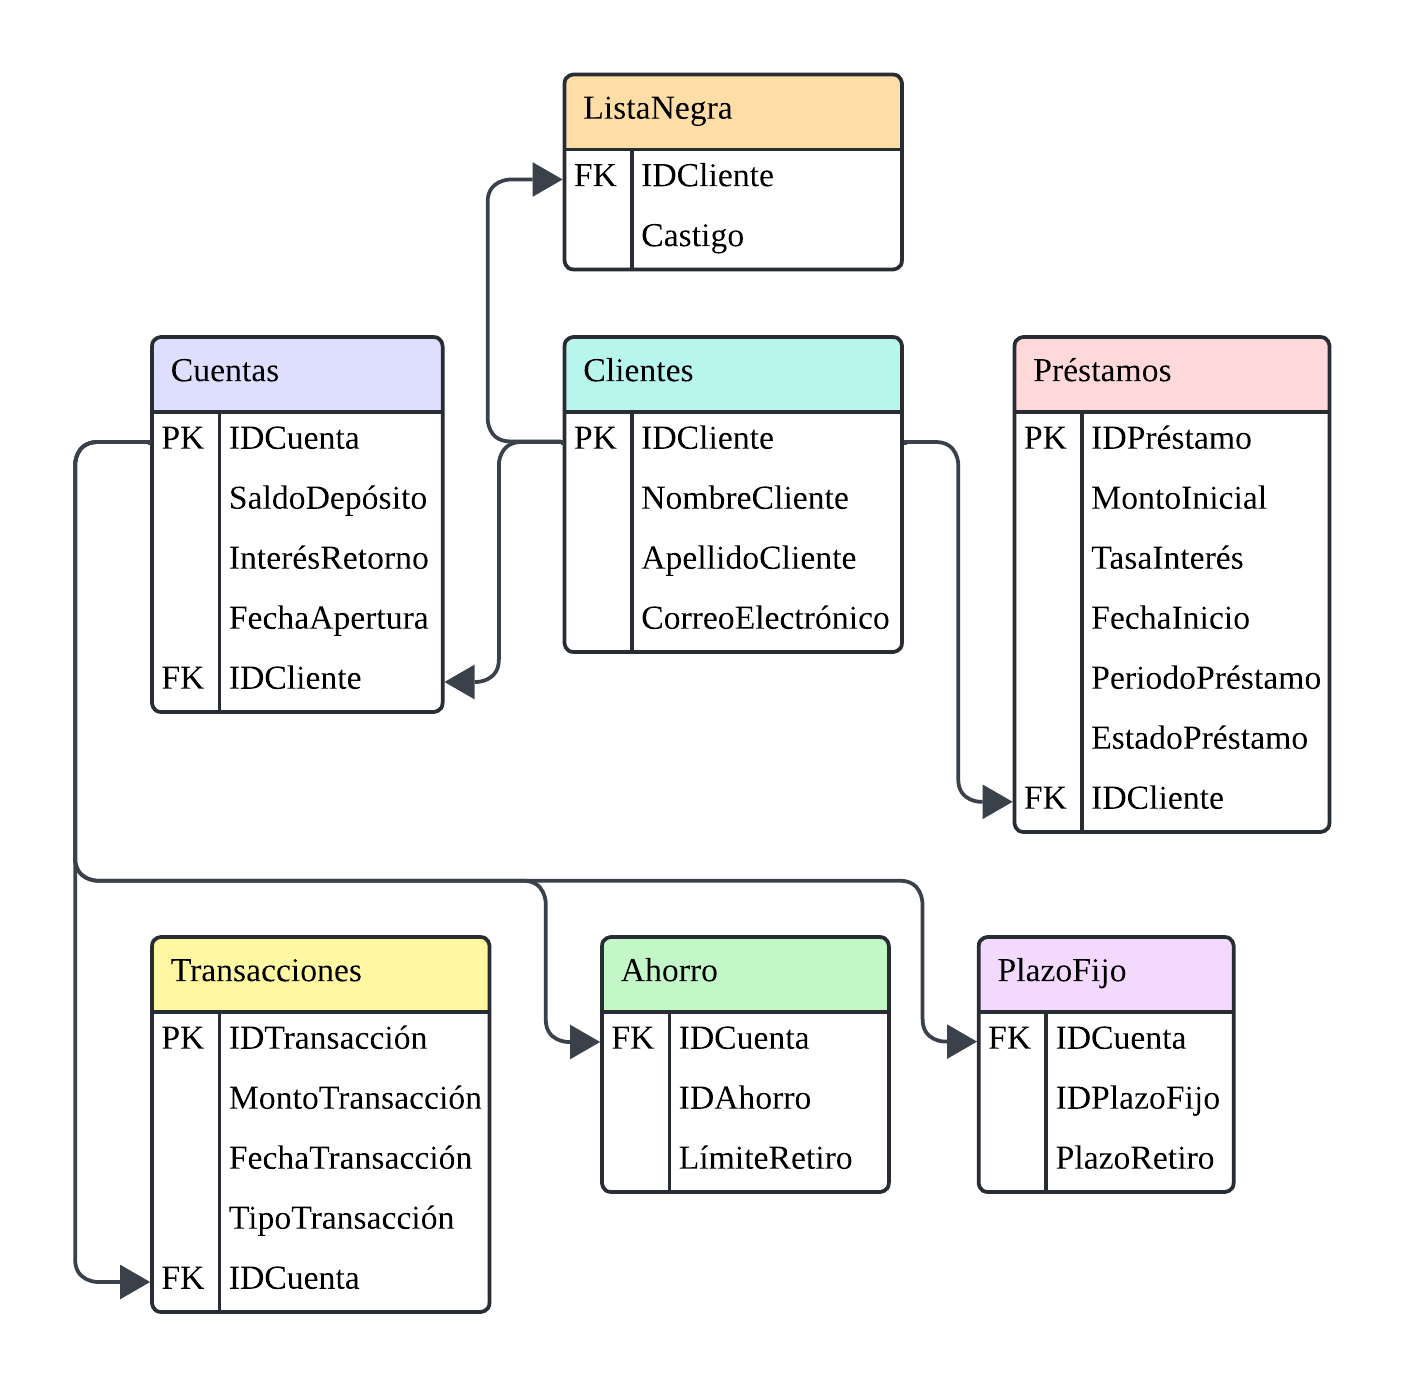
\includegraphics[scale = 0.3]{Imagenes/Diagramas/DR.png}
  \caption{Diagrama Relacional}
\end{figure}
\section{Creación de Base de Datos y Tablas}
\begin{figure}[H]
  \centering
  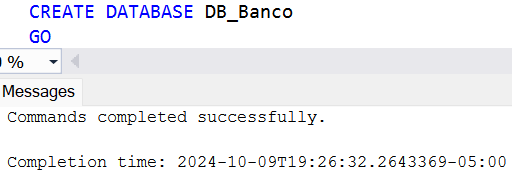
\includegraphics[scale = 0.6]{Imagenes/SQL/1.Crear_db/crear_db.png}
  \caption{Creación Base de Datos DB-Banco}
\end{figure}

\begin{figure}[H]
  \centering
  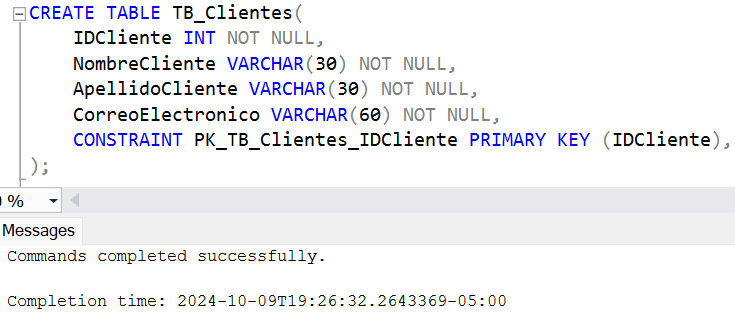
\includegraphics[scale = 0.5]{Imagenes/SQL/2.Crear_tablas/crear_tb_clientes.png}
  \caption{Creación de la tabla TB-Clientes}
\end{figure}

\begin{figure}[H]
  \centering
  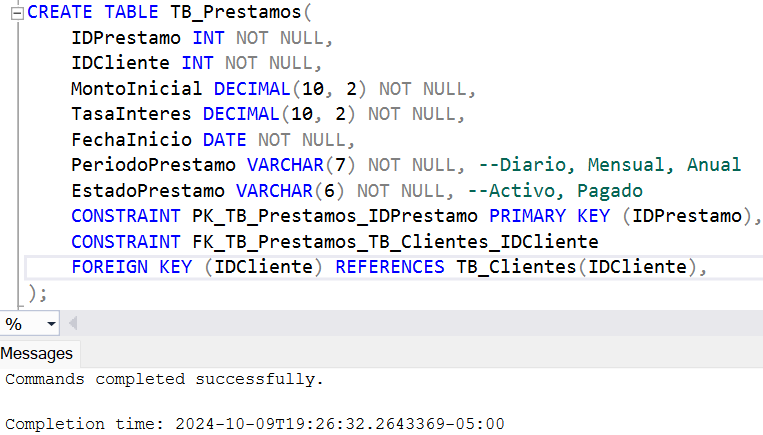
\includegraphics[scale = 0.5]{Imagenes/SQL/2.Crear_tablas/crear_tb_prestamos.png}
  \caption{Creación de la tabla TB-Prestamos}
\end{figure}

\begin{figure}[H]
  \centering
  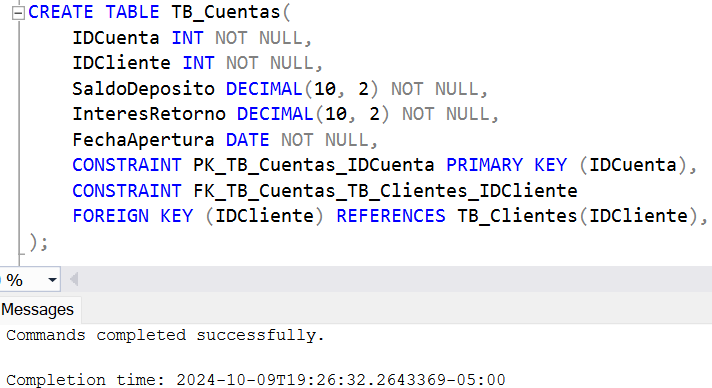
\includegraphics[scale = 0.6]{Imagenes/SQL/2.Crear_tablas/crear_tb_cuentas.png}
  \caption{Creación de la tabla TB-Cuentas}
\end{figure}

\begin{figure}[H]
  \centering
  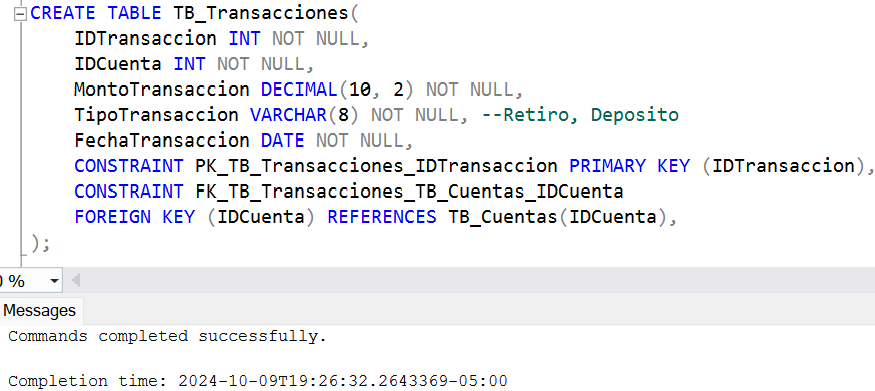
\includegraphics[scale = 0.6]{Imagenes/SQL/2.Crear_tablas/crear_tb_transacciones.png}
  \caption{Creación de la tabla TB-Transacciones}
\end{figure}

\begin{figure}[H]
  \centering
  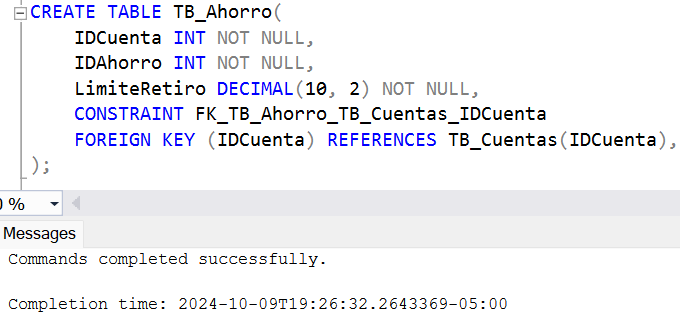
\includegraphics[scale = 0.6]{Imagenes/SQL/2.Crear_tablas/crear_tb_ahorro.png}
  \caption{Creación de la tabla TB-Ahorro}
\end{figure}

\begin{figure}[H]
  \centering
  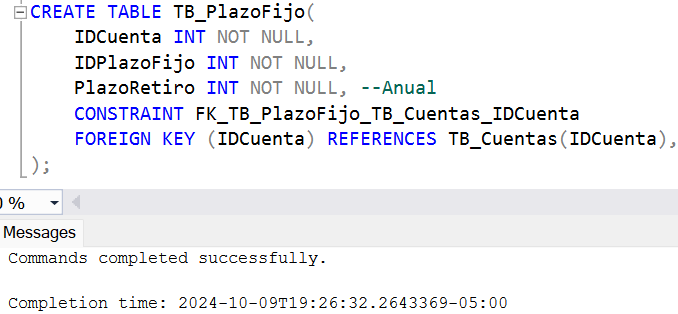
\includegraphics[scale = 0.6]{Imagenes/SQL/2.Crear_tablas/crear_tb_plazofijo.png}
  \caption{Creación de la tabla TB-PlazoFijo}
\end{figure}

\begin{figure}[H]
  \centering
  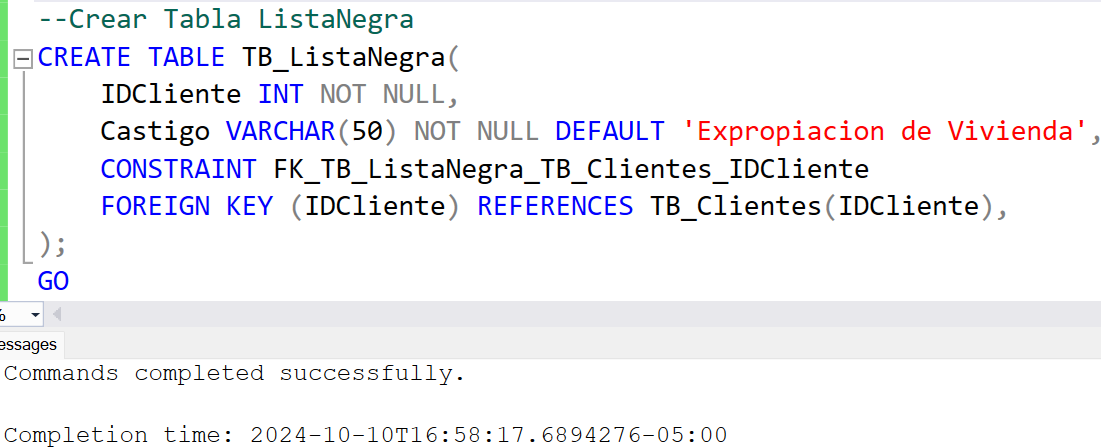
\includegraphics[scale = 0.5]{Imagenes/SQL/2.Crear_tablas/crear_tb_listanegra.png}
  \caption{Creación de la tabla TB-ListaNegra}
\end{figure}
\section{Creación de Triggers}
\begin{figure}[H]
  \centering
  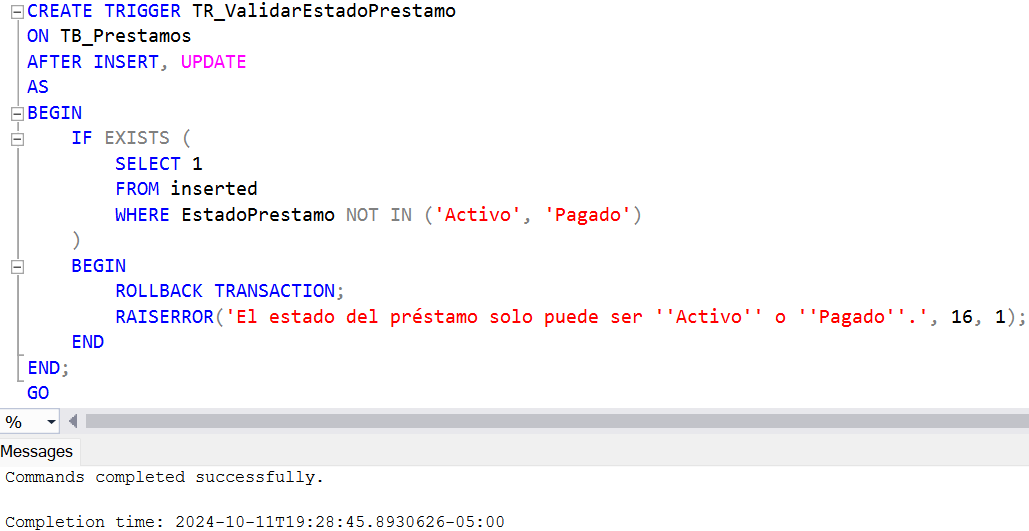
\includegraphics[scale = 0.5]{Imagenes/SQL/3.Triggers/TR_ValidarEstadoPrestamo.png}
  \caption{Creación Trigger TR-ValidarEstadoPrestamo}
\end{figure}

\begin{figure}[H]
  \centering
  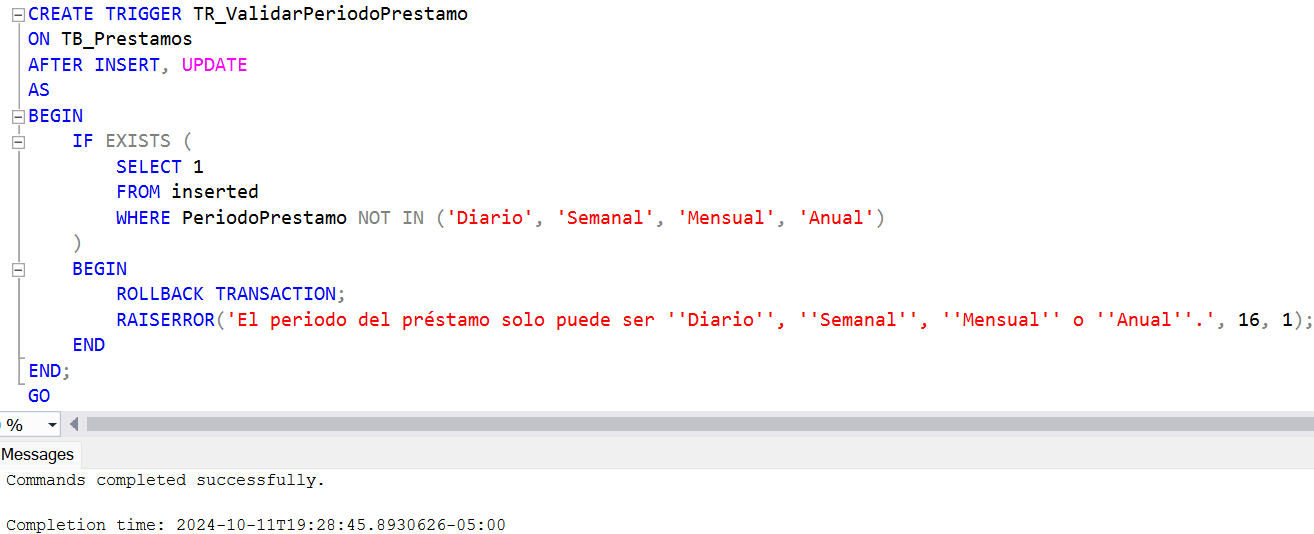
\includegraphics[scale = 0.4]{Imagenes/SQL/3.Triggers/TR_ValidarPeriodoPrestamo.png}
  \caption{Creación Trigger TR-ValidarPeriodoPrestamo}
\end{figure}

\begin{figure}[H]
  \centering
  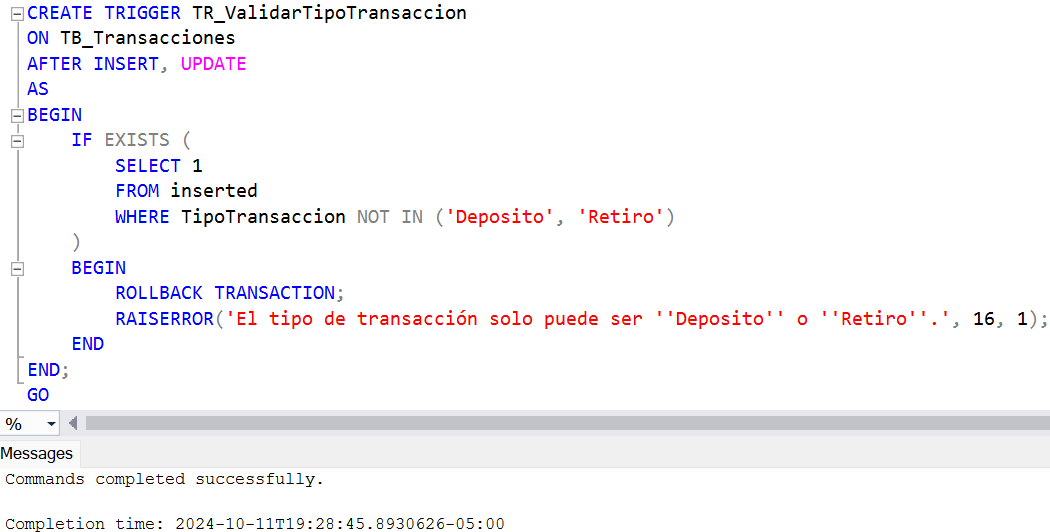
\includegraphics[scale = 0.4]{Imagenes/SQL/3.Triggers/TR_ValidarTipoTransaccion.png}
  \caption{Creación Trigger TR-ValidarTipoTransaccion}
\end{figure}

\begin{figure}[H]
  \centering
  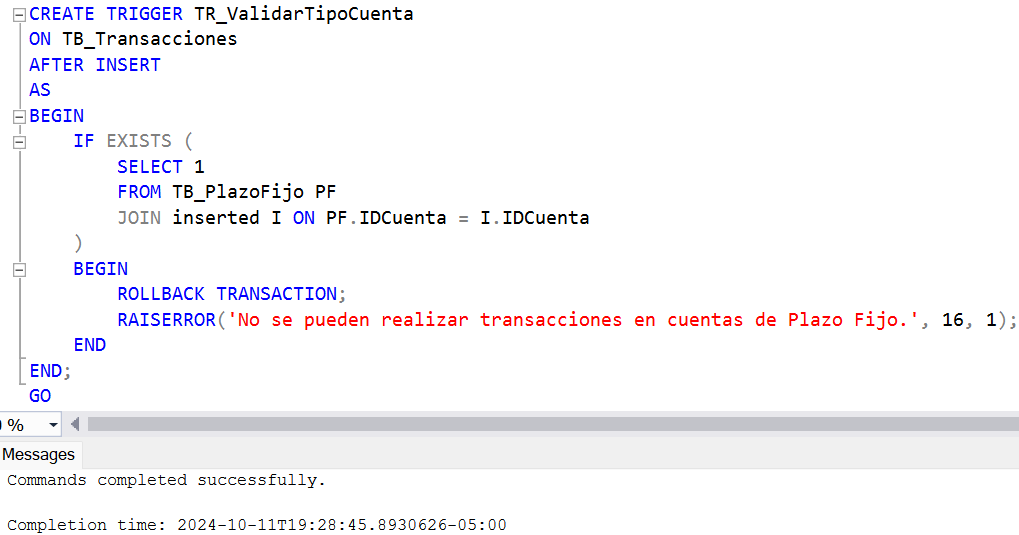
\includegraphics[scale = 0.4]{Imagenes/SQL/3.Triggers/TR_ValidarTipoCuenta.png}
  \caption{Creación Trigger TR-ValidarTipoCuenta}
\end{figure}

\begin{figure}[H]
  \centering
  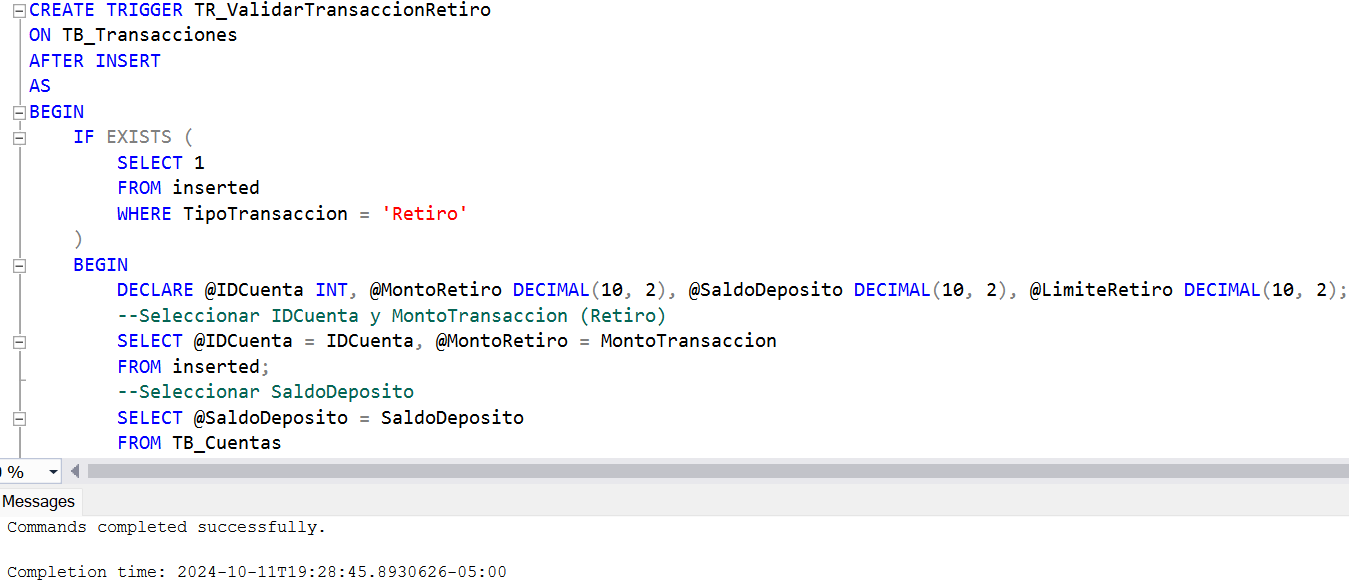
\includegraphics[scale = 0.3]{Imagenes/SQL/3.Triggers/TR_ValidarTransaccionRetiro.png}
  \caption{Creación Trigger TR-ValidarTransaccionRetiro}
\end{figure}

\begin{figure}[H]
  \centering
  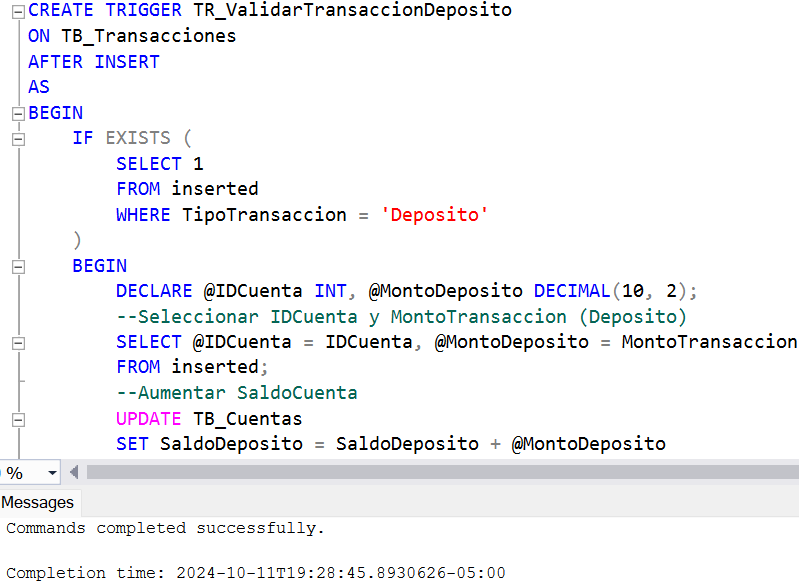
\includegraphics[scale = 0.4]{Imagenes/SQL/3.Triggers/TR_ValidarTransaccionDeposito.png}
  \caption{Creación Trigger TR-ValidarTransaccionDeposito}
\end{figure}

\begin{figure}[H]
  \centering
  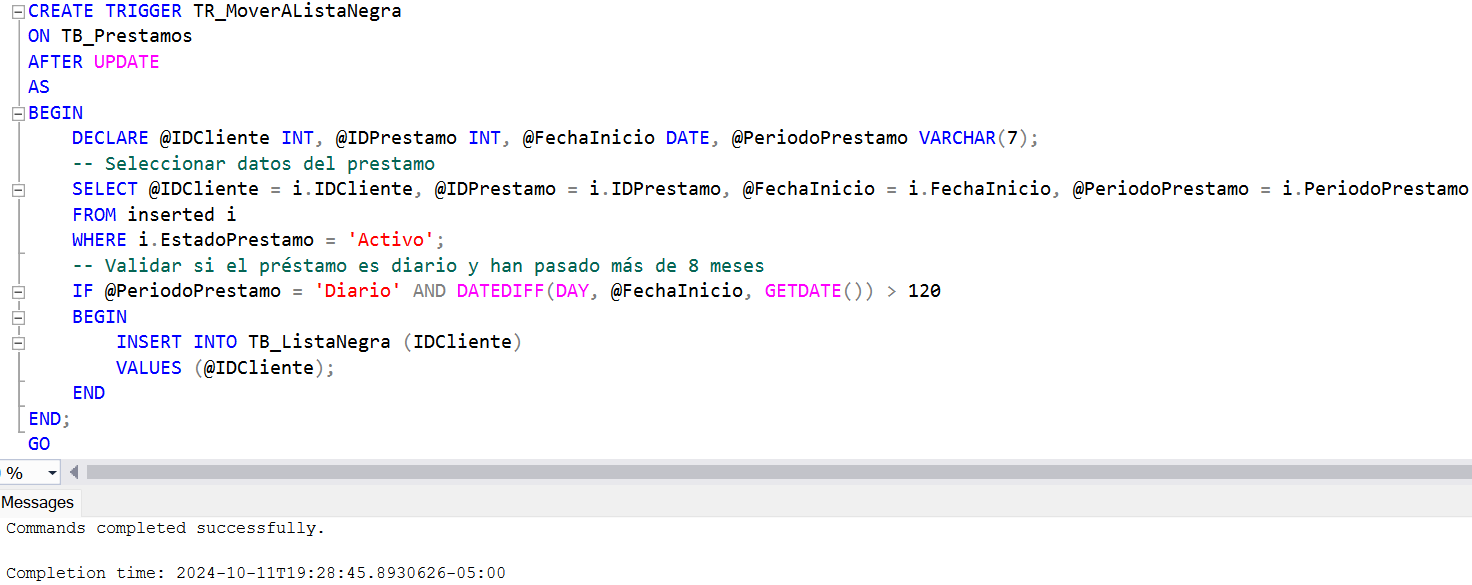
\includegraphics[scale = 0.3]{Imagenes/SQL/3.Triggers/TR_MoverAListaNegra.png}
  \caption{Creación Trigger TR-MoverAListaNegra}
\end{figure}
\section{Inserción de Registros}
\begin{figure}[H]
  \centering
  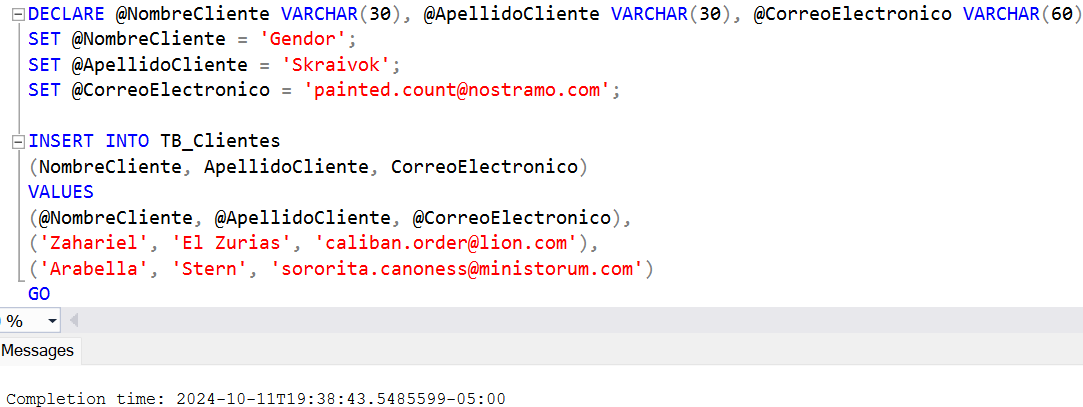
\includegraphics[scale = 0.5]{Imagenes/SQL/4.Insertar_registros/insertar_tb_clientes.png}
  \caption{Inserción registros Clientes}
\end{figure}

\begin{figure}[H]
  \centering
  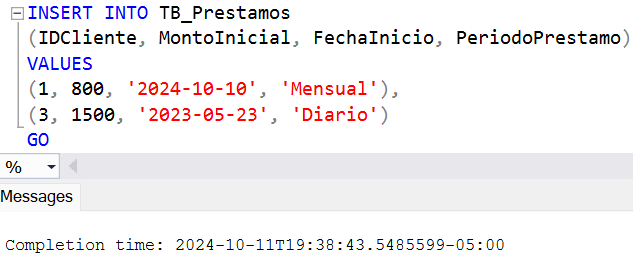
\includegraphics[scale = 0.5]{Imagenes/SQL/4.Insertar_registros/insertar_tb_prestamos.png}
  \caption{Inserción registros Prestamos}
\end{figure}

\begin{figure}[H]
  \centering
  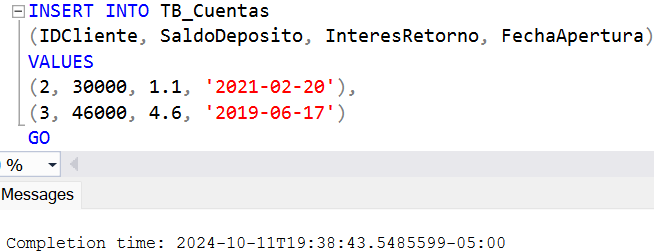
\includegraphics[scale = 0.5]{Imagenes/SQL/4.Insertar_registros/insertar_tb_cuentas.png}
  \caption{Inserción registros Cuentas}
\end{figure}

\begin{figure}[H]
  \centering
  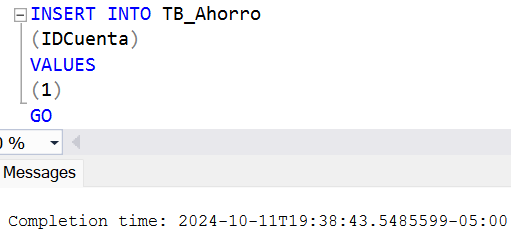
\includegraphics[scale = 0.5]{Imagenes/SQL/4.Insertar_registros/insertar_tb_ahorro.png}
  \caption{Inserción registros Ahorro}
\end{figure}

\begin{figure}[H]
  \centering
  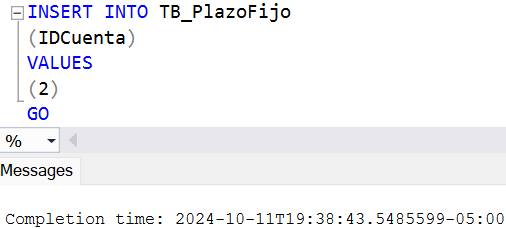
\includegraphics[scale = 0.5]{Imagenes/SQL/4.Insertar_registros/insertar_tb_plazofijo.png}
  \caption{Inserción registros PlazoFijo}
\end{figure}
\section{Probar Triggers}
\begin{figure}[H]
  \centering
  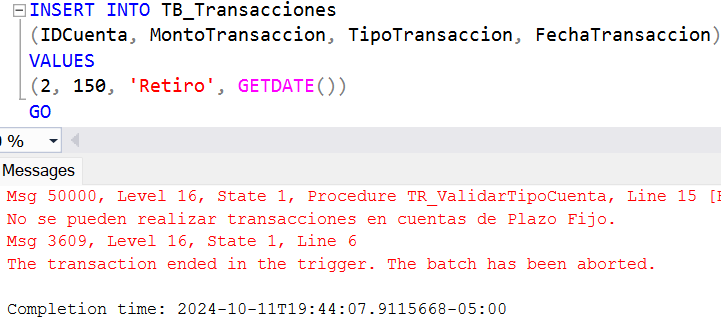
\includegraphics[scale = 0.5]{Imagenes/SQL/5.Ejercicios/restriccion_transaccion_plazofijo.png}
  \caption{Restricción Transacción PlazoFijo}
\end{figure}

\begin{figure}[H]
  \centering
  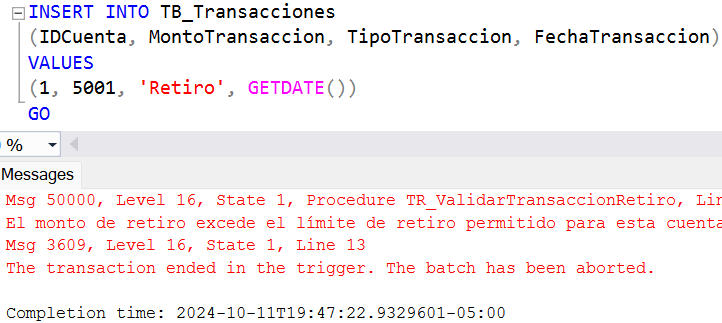
\includegraphics[scale = 0.5]{Imagenes/SQL/5.Ejercicios/restriccion_transaccion_limiteahorro.png}
  \caption{Restricción Transacción límite en Retiro}
\end{figure}

\begin{figure}[H]
  \centering
  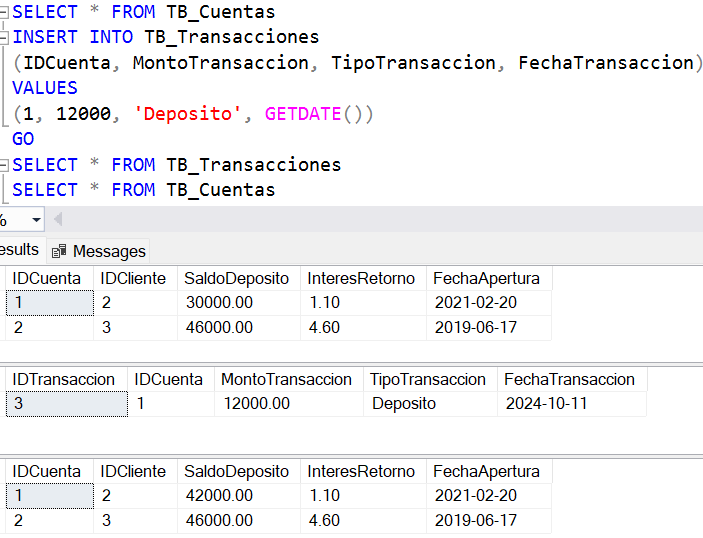
\includegraphics[scale = 0.5]{Imagenes/SQL/5.Ejercicios/activar_trigger_aumentodeposito.png}
  \caption{Activar Trigger aumento de Depósito}
\end{figure}

\begin{figure}[H]
  \centering
  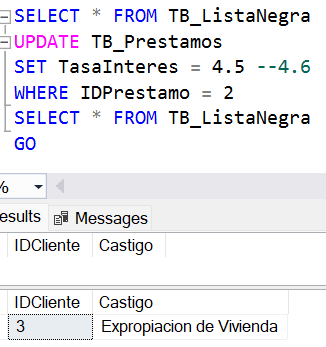
\includegraphics[scale = 0.5]{Imagenes/SQL/5.Ejercicios/activar_trigger_listanegra.png}
  \caption{Activar Trigger enviar a Lista Negra}
\end{figure}


\section{Ejercicios}
\begin{figure}[H]
  \centering
  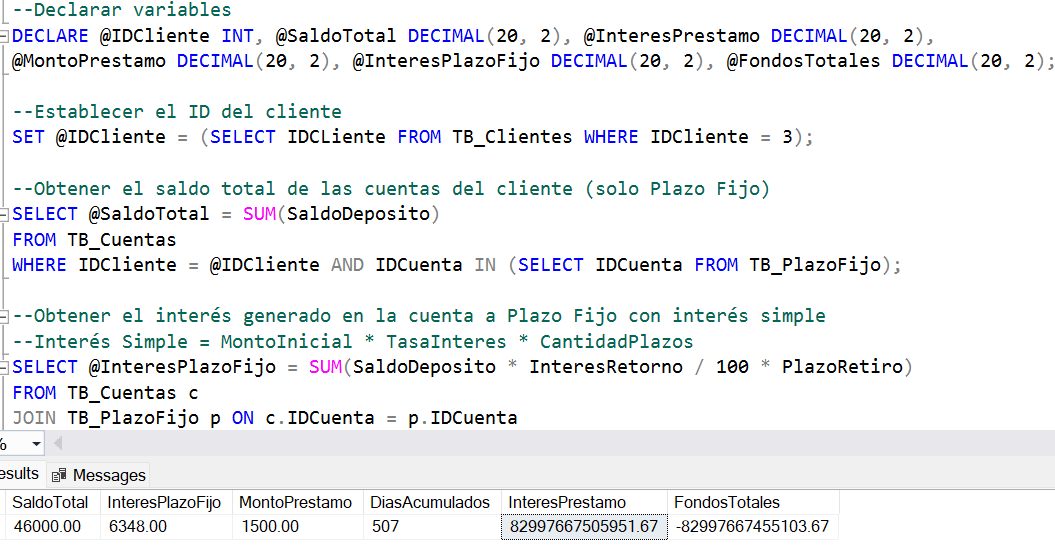
\includegraphics[scale = 0.5]{Imagenes/SQL/5.Ejercicios/fondos_totales.png}
  \caption{Ejercicio Fondos Totales}
\end{figure}
\end{document}